\documentclass[11pt]{article}
\usepackage{amsmath}
\usepackage{tikz}

\newcommand{\numpy}{{\tt numpy}}    % tt font for numpy

\topmargin -.5in
\textheight 9in
\oddsidemargin -.25in
\evensidemargin -.25in
\textwidth 7in

\begin{document}

% ========== Edit your name here
\author{bob the legend}
\title{POTD 538}
\maketitle

\medskip

% ========== Begin answering questions here
\begin{enumerate}

    \item
          First possible method



          \tikzset{every picture/.style={line width=0.75pt}} %set default line width to 0.75pt        
          \begin{figure}[h]
              \center
              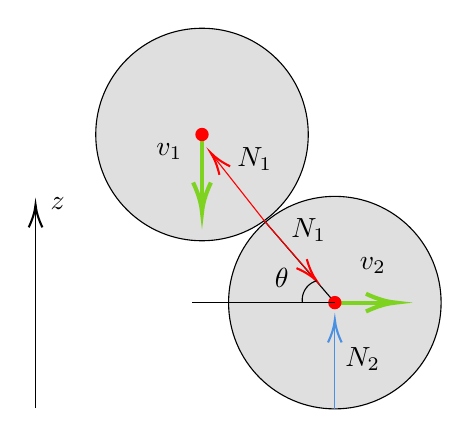
\begin{tikzpicture}[x=0.75pt,y=0.75pt,yscale=-1,xscale=1]
                  %uncomment if require: \path (0,300); %set diagram left start at 0, and has height of 300

                  %Shape: Circle [id:dp9632032114898363] 
                  \draw  [fill={rgb, 255:red, 223; green, 223; blue, 223 }  ,fill opacity=1 ] (312,177.2) .. controls (312,148.92) and (334.92,126) .. (363.2,126) .. controls (391.48,126) and (414.4,148.92) .. (414.4,177.2) .. controls (414.4,205.48) and (391.48,228.4) .. (363.2,228.4) .. controls (334.92,228.4) and (312,205.48) .. (312,177.2) -- cycle ;
                  %Straight Lines [id:da19424148333865587] 
                  \draw    (329.4,138) -- (363.2,177.2) ;
                  %Shape: Circle [id:dp828009152836988] 
                  \draw  [fill={rgb, 255:red, 223; green, 223; blue, 223 }  ,fill opacity=1 ] (248,96.2) .. controls (248,67.92) and (270.92,45) .. (299.2,45) .. controls (327.48,45) and (350.4,67.92) .. (350.4,96.2) .. controls (350.4,124.48) and (327.48,147.4) .. (299.2,147.4) .. controls (270.92,147.4) and (248,124.48) .. (248,96.2) -- cycle ;
                  %Straight Lines [id:da9789210903038281] 
                  \draw    (219,228) -- (219,132) ;
                  \draw [shift={(219,130)}, rotate = 450] [color={rgb, 255:red, 0; green, 0; blue, 0 }  ][line width=0.75]    (10.93,-3.29) .. controls (6.95,-1.4) and (3.31,-0.3) .. (0,0) .. controls (3.31,0.3) and (6.95,1.4) .. (10.93,3.29)   ;
                  %Straight Lines [id:da6327447573438989] 
                  \draw [color={rgb, 255:red, 255; green, 0; blue, 0 }  ,draw opacity=1 ]   (329.4,138) -- (304.64,106.57) ;
                  \draw [shift={(303.4,105)}, rotate = 411.77] [color={rgb, 255:red, 255; green, 0; blue, 0 }  ,draw opacity=1 ][line width=0.75]    (10.93,-3.29) .. controls (6.95,-1.4) and (3.31,-0.3) .. (0,0) .. controls (3.31,0.3) and (6.95,1.4) .. (10.93,3.29)   ;
                  %Straight Lines [id:da8701269618038006] 
                  \draw [color={rgb, 255:red, 255; green, 0; blue, 0 }  ,draw opacity=1 ]   (329.4,138) -- (353.09,165.17) ;
                  \draw [shift={(354.4,166.68)}, rotate = 228.92000000000002] [color={rgb, 255:red, 255; green, 0; blue, 0 }  ,draw opacity=1 ][line width=0.75]    (10.93,-3.29) .. controls (6.95,-1.4) and (3.31,-0.3) .. (0,0) .. controls (3.31,0.3) and (6.95,1.4) .. (10.93,3.29)   ;
                  %Straight Lines [id:da6975293187447933] 
                  \draw [color={rgb, 255:red, 74; green, 144; blue, 226 }  ,draw opacity=1 ]   (363.2,228.4) -- (363.2,187.44) ;
                  \draw [shift={(363.2,185.44)}, rotate = 450] [color={rgb, 255:red, 74; green, 144; blue, 226 }  ,draw opacity=1 ][line width=0.75]    (10.93,-3.29) .. controls (6.95,-1.4) and (3.31,-0.3) .. (0,0) .. controls (3.31,0.3) and (6.95,1.4) .. (10.93,3.29)   ;
                  %Straight Lines [id:da8075814011334781] 
                  \draw [color={rgb, 255:red, 126; green, 211; blue, 33 }  ,draw opacity=1 ][line width=1.5]    (299.2,96.2) -- (299.2,130.56) ;
                  \draw [shift={(299.2,133.56)}, rotate = 270] [color={rgb, 255:red, 126; green, 211; blue, 33 }  ,draw opacity=1 ][line width=1.5]    (14.21,-4.28) .. controls (9.04,-1.82) and (4.3,-0.39) .. (0,0) .. controls (4.3,0.39) and (9.04,1.82) .. (14.21,4.28)   ;
                  %Straight Lines [id:da6634036078325487] 
                  \draw [color={rgb, 255:red, 126; green, 211; blue, 33 }  ,draw opacity=1 ][line width=1.5]    (363.2,177.2) -- (389.4,177.2) ;
                  \draw [shift={(392.4,177.2)}, rotate = 180] [color={rgb, 255:red, 126; green, 211; blue, 33 }  ,draw opacity=1 ][line width=1.5]    (14.21,-4.28) .. controls (9.04,-1.82) and (4.3,-0.39) .. (0,0) .. controls (4.3,0.39) and (9.04,1.82) .. (14.21,4.28)   ;
                  %Shape: Circle [id:dp7245157625352985] 
                  \draw  [draw opacity=0][fill={rgb, 255:red, 255; green, 0; blue, 0 }  ,fill opacity=1 ] (295.99,96.2) .. controls (295.99,94.43) and (297.43,92.99) .. (299.2,92.99) .. controls (300.97,92.99) and (302.41,94.43) .. (302.41,96.2) .. controls (302.41,97.97) and (300.97,99.41) .. (299.2,99.41) .. controls (297.43,99.41) and (295.99,97.97) .. (295.99,96.2) -- cycle ;
                  %Shape: Circle [id:dp5386224150342513] 
                  \draw  [draw opacity=0][fill={rgb, 255:red, 255; green, 0; blue, 0 }  ,fill opacity=1 ] (359.99,177.2) .. controls (359.99,175.43) and (361.43,173.99) .. (363.2,173.99) .. controls (364.97,173.99) and (366.41,175.43) .. (366.41,177.2) .. controls (366.41,178.97) and (364.97,180.41) .. (363.2,180.41) .. controls (361.43,180.41) and (359.99,178.97) .. (359.99,177.2) -- cycle ;
                  %Straight Lines [id:da8942428050350879] 
                  \draw    (294.4,177.2) -- (363.2,177.2) ;
                  %Shape: Arc [id:dp265111753111414] 
                  \draw  [draw opacity=0] (347.53,177.02) .. controls (347.47,176.51) and (347.45,175.98) .. (347.48,175.44) .. controls (347.68,171.23) and (350.57,167.79) .. (354.4,166.68) -- (357.07,175.91) -- cycle ; \draw   (347.53,177.02) .. controls (347.47,176.51) and (347.45,175.98) .. (347.48,175.44) .. controls (347.68,171.23) and (350.57,167.79) .. (354.4,166.68) ;

                  % Text Node
                  \draw (225,125.4) node [anchor=north west][inner sep=0.75pt]    {$z$};
                  % Text Node
                  \draw (315,101.4) node [anchor=north west][inner sep=0.75pt]    {$N_{1}$};
                  % Text Node
                  \draw (341,135.4) node [anchor=north west][inner sep=0.75pt]    {$N_{1}$};
                  % Text Node
                  \draw (367,197.4) node [anchor=north west][inner sep=0.75pt]    {$N_{2}$};
                  % Text Node
                  \draw (276,99.4) node [anchor=north west][inner sep=0.75pt]    {$v_{1}$};
                  % Text Node
                  \draw (374,154.4) node [anchor=north west][inner sep=0.75pt]    {$v_{2}$};
                  % Text Node
                  \draw (333,159.4) node [anchor=north west][inner sep=0.75pt]    {$\theta $};


              \end{tikzpicture}
          \end{figure}

          Relating velocity of top and bottom cylinders
          \begin{equation}
              v_2=v_1 \tan \theta
          \end{equation}

          Relative velocity $v_{2,1}$ where $v_2 -v_{2,1} = v_1$
          \begin{equation}
              v_{2,1}=v_1\sqrt{\tan^2\theta-1}
          \end{equation}

          So to find rate of change of $\theta$, just let $v_{2,1}=r\frac{d\theta}{dt}$ since $v_{2,1}$ always points in the tangential direction and rate of change of $\theta$ is essentially just angular velocity of the bottom cylinders around the top one? so we get:

          \begin{equation}
              \omega=\frac{v_1\sqrt{\tan^2\theta-1}}{r}
          \end{equation}

          differentiating both sides to get $\frac{d^2 \theta}{dt^2}$
          \begin{equation}
              \frac{d^2 \theta}{dt^2}=\frac{\sqrt{\tan^2\theta-1}}{r}\frac{dv_1}{dt}+v_1\frac{d(\sqrt{\tan^2\theta-1})}{dt}
          \end{equation}
          where $\frac{d\theta}{dt}=\omega$

          so how to find $dv_1/dt$? (just $a_1$ where $a$ refers to acceleration)
          Write out $F=ma$ for both the top and bottom

          \begin{center}
              \begin{tabular}{p{5cm}p{5cm}}
                  \begin{equation}
                      mg-3N\sin\theta=ma_1
                  \end{equation}
                   &
                  \begin{equation}
                      N\cos\theta=ma_1\tan\theta
                  \end{equation}
              \end{tabular}
          \end{center}

          Solving for $a_1$ gives us
          \begin{equation}
              a=\frac{g}{1+3 \tan^2 \theta}
          \end{equation}

          Final solution for $\frac{d^2\theta}{dt^2}$

          \begin{equation}
              \boxed{
              \frac{d^2\theta}{dt^2}=\frac{g}{1+3 \tan^2 \theta}\frac{\sqrt{\tan^2\theta-1}}{r}+\frac{1}{2} (\tan^2\theta-1)^{-\frac{1}{2}}2 \sec^2 \theta \tan \theta r\omega^2}
          \end{equation}

\end{enumerate}

\end{document}
\grid
\grid